\documentclass[letterpaper, 12pt]{article}
\usepackage[top=.5in,bottom=.5in,left=.75in,right=.75in,headheight=30pt, % as per the warning by fancyhdr
includehead,includefoot,
heightrounded, % to avoid spurious underfull messages
]{geometry}
\addtolength{\topmargin}{-.25in}
\usepackage{fancyhdr}
\usepackage{cancel}
\usepackage{gensymb}
\usepackage{xcolor}
\usepackage{tikz}
\usetikzlibrary{angles, quotes}
\usepackage{amssymb}
\pagestyle{fancy}
\usepackage{graphicx}
\usepackage{lastpage}
\usepackage{multicol}
\newcommand{\assnum}{Assignment 0.03}
\newcommand{\assname}{Trigonometry Review}

\begin{document}
\fancyhead[l]{	\includegraphics[height=0.5in]{../Logo/sp.png} Name:}

\fancyfoot[c]{\thepage\ of \pageref{LastPage}}
\fancyfoot[r]{\assnum}	


\begin{center} \assnum{} - \assname{}
\end{center}





\begin{enumerate}
	\item Identify the opposite, adjacent, and hypotenuse of each of the following triangles:
	
\begin{tabular}{ c c c c}
	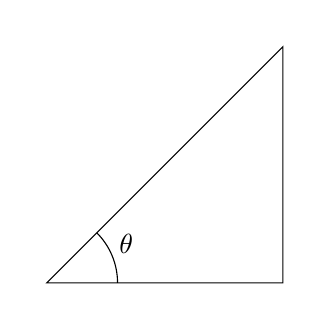
\begin{tikzpicture}
		\draw (0,0) node[anchor=east]{}
		-- (3,0) node[anchor=north]{}
		-- (3,3) node[anchor=south]{}
		-- cycle;
			\draw (.9,0) arc (0:45:.9) ;
		\draw (.8,.5) -- (.8,.5) node[anchor=west] {$\theta$};
		
	\end{tikzpicture} & 
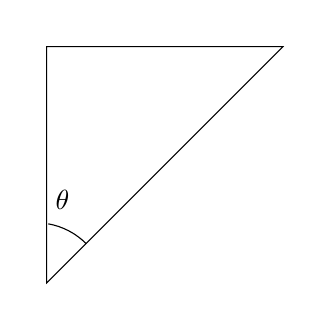
\begin{tikzpicture}
	\draw (0,0) node[anchor=east]{}
	-- (0,-3) node[anchor=north]{}
	-- (3,0) node[anchor=south]{}
	-- cycle;
	\draw (.5,-2.5) arc (45:80:.9) ;
	\draw (.2,-1.7) -- (.2,-1.7) node[anchor=north] {$\theta$};
	
\end{tikzpicture}& 
\begin{tikzpicture}
	\draw (0,0) node[anchor=east]{}
	-- (3,-3) node[anchor=north]{}
	-- (3,0) node[anchor=south]{}
	-- cycle;
	\draw (.5,-.50) arc (-45:-10:.9) ;
	\draw (.85,-.1) -- (.85,-.1) node[anchor=north] {$\theta$};
	
\end{tikzpicture}


& 	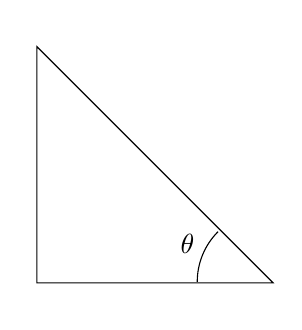
\begin{tikzpicture}
	\draw (0,0) node[anchor=east]{}
	-- (-3,0) node[anchor=north]{}
	-- (-3,3) node[anchor=south]{}
	-- cycle;
	\draw (-.7,.65) arc (135:180:.9) ;
	\draw (-1.3,.5) -- (-1.3,.5) node[anchor=west] {$\theta$};
	
\end{tikzpicture}
\end{tabular}


	\item Calculate the length of each side of the following triangles (not drawn to scale):
	
\begin{tabular}{c c}
	\begin{tikzpicture}
		\draw (0,0) node[anchor=east]{}
		-- (-5,0) node[anchor=north]{}
		-- (-5,3) node[anchor=south]{}
		-- cycle;
		\draw (-.7,.4) arc (155:180:.9) ;
		\draw (-1.5,.2) -- (-1.5,.2) node[anchor=west] {$25 \degree$};
		\draw (-1.9,1.5) -- (-1.9,1.5) node[anchor=south] {$6$ m};
		
	\end{tikzpicture}
	& \hspace{0.5in}
		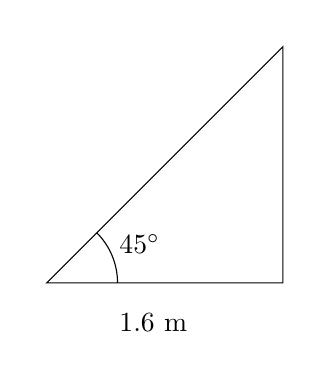
\begin{tikzpicture}
		\draw (0,0) node[anchor=east]{}
		-- (3,0) node[anchor=north]{}
		-- (3,3) node[anchor=south]{}
		-- cycle;
		\draw (.9,0) arc (0:45:.9) ;
		\draw (.8,.5) -- (.8,.5) node[anchor=west] {$45 \degree$};
		\draw (.8,-.5) -- (.8,-.5) node[anchor=west] {$1.6$ m};
	\end{tikzpicture} 
	
\end{tabular}
	

\item Ivan is walking across a field.  He walks 6000m in 40 minutes, at a 35° angle south of west.  
\begin{enumerate}
	\item Draw a diagram of the situation.
	\vspace{.9 in}
	\item How far west is Ivan from where he started?
	\vspace{0.4 in}
	\item How far south is Ivan from where he started?
	\vspace{0.4 in}
	\item How fast was Ivan walking?
	\vspace{0.4 in}
	\item How fast was Ivan moving to the west?  
	\vspace{0.4 in}	
	\item How fast was Ivan moving to the south?
	
\end{enumerate}


\item Calculate the indicated angle for each triangle:

\begin{tabular}{ c c c }
	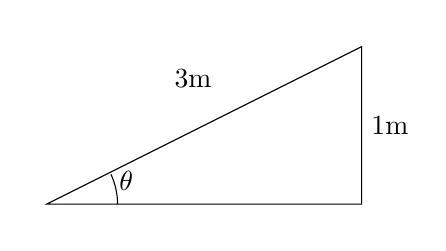
\begin{tikzpicture}
		\draw (0,0) node[anchor=east]{}
		-- (4,0) node[anchor=north]{}
		-- (4,2) node[anchor=south]{}
		-- cycle;
		\draw (.9,0) arc (0:25:.9) ;
		\draw (.8,.3) -- (.8,.3) node[anchor=west] {$\theta$};
		\draw (4,1) -- (4,1) node[anchor=west] {$1$m};
		\draw (1.5,1.6) -- (1.5,1.6) node[anchor=west] {$3$m};
	\end{tikzpicture} & 
\hspace{0.25 in}
	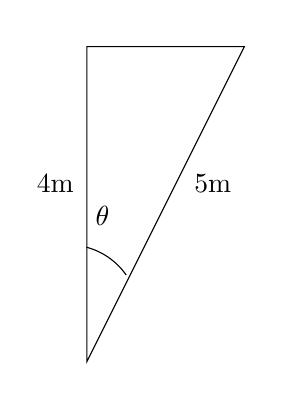
\begin{tikzpicture}
		\draw (0,0) node[anchor=east]{}
		-- (0,-4) node[anchor=north]{}
		-- (2,0) node[anchor=south]{}
		-- cycle;
		\draw (.5,-2.9) arc (35:75:.9) ;
		\draw (.2,-1.9) -- (.2,-1.9) node[anchor=north] {$\theta$};
		\draw (-.4,-1.5) -- (-.4,-1.5) node[anchor=north] {$4$m};
		\draw (1.6,-1.5) -- (1.6,-1.5) node[anchor=north] {$5$m};
		
		
	\end{tikzpicture}& 
\hspace{0.25 in}
	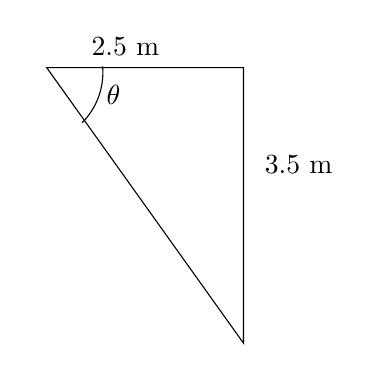
\begin{tikzpicture}
		\draw (0,0) node[anchor=east]{}
		-- (2.5,-3.5) node[anchor=north]{}
		-- (2.5,0) node[anchor=south]{}
		-- cycle;
		\draw (.45,-.7) arc (-45:5:.9) ;
		\draw (.85,-.1) -- (.85,-.1) node[anchor=north] {$\theta$};
		\draw (1,0.5) -- (1,0.5) node[anchor=north] {$2.5$ m};
		\draw (3.2,-1) -- (3.2,-1) node[anchor=north] {$3.5$ m};
		
	\end{tikzpicture}
\end{tabular}


\item Angel is hiking in the desert, where he walks 2 miles to the east, then 1 miles north.  
\begin{enumerate}
	\item Draw a diagram of the situation.
	\vspace{1 in}
	\item How far is Angel from where he started?
	\vspace{0.4 in} 
	\item Because he has been gone for so long, a search-and-rescue helicopter is dispatched to find Angel.  What angle (measured from east) should the helicopter pilot fly at to find him?
	\vspace{0.4 in}
\end{enumerate}

\item Hazel is flying in a plane at 350 m/s to the north.  The wind is blowing at 120 m/s to the east. 
\begin{enumerate}
	\item Draw a diagram of the situation.
	\vspace{1 in}
	\item What is Hazel’s resultant speed?
	\vspace{0.4 in}
	\item What angle will Hazel’s plane go (measured from north)?
	
\end{enumerate}




 



\end{enumerate}
\end{document}
